
\documentclass[journal,onecolumn,12pt]{IEEEtran}

\usepackage{cite}      % Written by Donald Arseneau
\usepackage{graphicx}  % Written by David Carlisle and Sebastian Rahtz
\usepackage{psfrag}    % Written by Craig Barratt, Michael C. Grant,
\usepackage{subfigure} % Written by Steven Douglas Cochran
\usepackage{url}       % Written by Donald Arseneau
\usepackage{amsmath}   % From the American Mathematical Society
\usepackage{amsfonts}
\interdisplaylinepenalty=2500
\usepackage{array}
\usepackage[hypertex]{hyperref}
\hyphenation{op-tical net-works semi-conduc-tor}

\newcommand{\epsfig}[5]{
 \begin{figure}[#4!]
   \begin{center}
    \includegraphics[width=#5\columnwidth]{#1}
    \caption{{\sl #2}\label{#3}}
   \end{center}
 \end{figure}}

\linespread{2}

\begin{document}
\title{High Performance Computing {MRI} Simulations}

\author{Tony~St\"ocker,~Kaveh Vahedipour,~and~N.~Jon~Shah
\thanks{All authors are with the Institute of Neuroscience and Biophysics,
        Forschungszentrum J\"ulich GmbH, 52425 J\"ulich, Germany.
	Corresponding Author: T.~St\"ocker, t.stoecker@fz-juelich.de}}
\markboth{Journal of \LaTeX\ Class Files,~Vol.~X, No.~XX,~November~200X}{St\"ocker \MakeLowercase{\textit{et al.}}: Bare Demo of IEEEtran.cls for Journals}

\maketitle

\begin{abstract}
MRI simulations are needed in many cases and deliver many advantages over real systems. Safety considerations for human
subjects as well as for the MRI hardware suggest the use of simulations prior to the implementation of new processes on
real MRI hardware. Likewise, the work involved in implementing new ideas on MRI scanners may require thorough
simulations.

A new open source software project is presented -- JEMRIS, the ``J\"ulich Extensible MRI Simulator'' -- which provides
an efficient, general, versatile, and extensible MRI sequence development and simulation environment for the MRI physics
and medical image processing community. The development was driven by the desire to achive three major goals: first,
generality of simulated 3D MRI experiments reflecting modern MRI system hardware was most important, even at the expense
of computational burden. Second, the user interface should be simple to use but present few limitations. JEMRIS
does not provide predefined experimental set-ups (such as MRI sequences) but allows rapid GUI-based implementation of
nearly arbitrary complex experimental conditions and sequences. Finally, the incorporated physical model, sequence
framework, as well as the simulated samples should be reconfigurable, replaceable and extensible. The present manuscript
describes the concepts, methods, and performance of the software. In particular, based on the description herein, the
community can test, work with, and contribute to future developments.

\end{abstract}

\begin{keywords}
MRI simulation, Bloch equations, sequence development, high performance computing,
object-oriented design patterns
\end{keywords}


\section{Introduction}
Numerical simulation of MRI experiments, based on the Bloch equation, is an essential tool for a variety of different
research directions. In the field of pulse sequence optimisation, e.g.~for artefact detection and elimination,
simulations allow differentiation between effects arising principally from MRI physics and those due to hardware
imperfections. If the simulation environment is able to simulate hardware malfunction, then the results may be used for
the optimisation of the hardware itself. Another prominent application is the design of specialised RF pulses which is
often based on numerical simulations of the excitation process. In general, the interpretation and validation of
experimental results benefits from comparisons to simulated data, which is especially important in the context of
MRI-compatible sample development, e.g.~for the development of implants. Another important application is image
generation for the purposes of medical image processing -- here, complete control of the properties of the input data
allows a tailored design of image processing algorithms. Last but not least, MRI simulations give an extraordinary
insight to the complex physics of MR signal generation and the encoding of spatial information with imaging
gradients. Especially interesting is the observation of aspects which are hidden in the real experiment -- for instance
the time evolution of the longitudinal magnetisation. With regard to the latter point, therefore, controlled numerical
MRI experiments are also highly valuable for educational purpose. 

In its most general form, numerical simulation of an MRI experiment is a demanding task. This is due to the fact that a
huge spin ensemble has to be Simulated in order to obtain realistic results. To overcome this, several published
approaches reduce the problem size in different ways. The most prominent method is to consider cases in which analytical
solutions to the problem exist \cite{kwan,benoit,yoder}. In case of simultaneous RF excitation and time varying gradient
fields no general analytical solution exists and, thus, the important field of selective excitation cannot be studied
with analytical approaches. In the past, numerical solutions have also been considered \cite{summers,olsson} but hard-
and software architectures pertaining at that time allowed only limited simulations of small spin systems with reduced
flexibility in set-up and extensibility of the numerical experiments. Apart from the computational demand, the
complexity of the MRI imaging sequence is also an obstacle. The difficulty of MRI sequence implementation using the
software environments of commercial MRI scanners -- painfully experienced by many researchers and pulse programmers --
can be significantly reduced with appropriate software design patterns \cite{joch}. Also, a multi-purpose MRI
simulation environment should provide such functionality for rapid sequence prototyping. Otherwise, it will be of
limited interest only. However, providing an easy-to-use framework should by no means increase the internal complexity
thereof. This would reduce the possibility of extending and changing the framework and again result in limited usability
for tailored applications. 

The JEMRIS project was initiated taking all of the aforementioned considerations into account. The original driving
forces for JEMRIS where: i) the need for accurate MRI simulations in the most general case of non-interacting classical
spins (e.g.~for the design of long RF pulses, where simultaneously, gradient fields and relaxation need to be taken into
account); ii) the availability of high performance computing (HPC) at the authors' institution; and iii) the lack of a
freely available software project capable of, or extendable to i). Compared to previously published approaches in the
field of MRI simulations, JEMRIS distinguishes itself in several aspects. An approximate comparison may be supported by
listing the most important features:

\begin{itemize}
 \item A highly optimised library for numerical solutions of differential equations is utilised. JEMRIS thus provides
   exact 3D MRI simulation results in cases where no analytical solution is available. For example, in case of simple
   slice selection where RF pulses and gradients are applied simultaneously. It is thus well suited, and has been
   successfully applied, for designing multi-channel 3D spatially selective excitations.
 \item JEMRIS can deal with arbitrary RF and gradient shapes, arbitrary multi-channel Tx-Rx coil geometries and
   configurations, as well as many important physical concepts such as random and deterministic off-resonance effects,
   concomitant fields, nonlinear gradients, etc.
 \item Symbolic mathematical calculations are supported by means of a dedicated library. Thus, many extensions are
   readily available with no additional programming involved, e.g.~the definition of arbitrary analytical pulse shapes
   within the MRI sequence.
 \item The core simulation routines take advantage of massive parallel processing and are available on different
   hardware architectures. JEMRIS can perform simulations on reasonable sample sizes and experiment setups on
   single-core hardware. It has also been extensively used for simulations on small-scale clusters. Further, JEMRIS has
   also been deployed on massively parallel setups such as JUGENE, the world’s fifth fastest civilian supercomputer with
   65536 computer cores and more than 220 T-FLOPS peak performance.
 \item The code is based on well studied object-oriented software design patterns tailored for MRI applications as well
   as for extending the framework.
 \item The software is easy to use. A user interface is provided with which all simulation parameters are configured,
   including nearly arbitrary complex MRI sequences.
 \item JEMRIS is open source and the community is encouraged to make future contributions to the project under {\sf
   www.jemris.org}. It has been coded only in ANSI C++, and it has been successfully tested on Linux, Windows and Mac OS
   X.
\end{itemize}

Thus, in contrast to the commonly available simulation environments for MRI, JEMRIS offers a highly optimized
computational platform for the most general numerical solution of the Bloch equations of non-interacting classical
spins.  JEMRIS does not place limitations on MR sequence design or sample size besides those set by the computation
hardware. Furthermore, JEMRIS leaves room for future expansions of the underlying framework in a multitude of imaginable
directions, be they the introduction of dynamic samples, interaction of spins, additional physical models, or numerical
differential equation integrators. In its current form, JEMRIS offers great flexibility due to the implementation of
symbolic mathematics for almost all parameters involved in the simulation process.

The present manuscript summarises the functionality and possibilities provided by the JEMRIS framework. The Physical
Concepts section briefly introduces the physical models on which JEMRIS is based. A conceptual description of the actual
implementation is given in the Software Design section -- here, basic knowledge of object-oriented programming and XML
data structures is helpful to aid understanding. Performance benchmarks and basic examples are given in the Results section.


%%%%%%%%%%%%%%%%%%%%%%%%%%%%%%%%%%%%%%%%%%%%%%%%%%%%%%%

\section{Physical Concepts}

The simulator is based on a classical description of MRI physics as described by the Bloch equations. It provides an
exact concept for the description of non-interacting spin isochromats under the influence of an external magnetic field
with a strong static component as well as a temporally and spatially varying field along the same direction (the imaging
gradients) and rapidly varying components in orthogonal directions (the RF field). A mathematical and numerical
treatment is greatly simplified in the rotating frame of reference, in which the effect of the main field can be ignored
since the coordinate system rotates with the spin precession. Then, the magnetic field at time $t$ and position ${\bf
  r}$ is given by:

\begin{eqnarray}
        {\bf B}({\bf r},t) & = & [{\bf G}(t)\cdot{\bf r}+\Delta\omega({\bf r},t)]{\bf e}_z \nonumber \\
                           &   & \,+\,\sum_{n=1}^{N}\left(B_{1x}^n({\bf r},t){\bf e}_x+B_{1y}^n({\bf r},t){\bf e}_y\right)\,, \label{eq:field}
\end{eqnarray}

where ${\bf e}_{x,y,z}$ denote unit Cartesian vectors. $B_{1x,y}^n({\bf r},t)$ are the excitation radio-frequency (RF)
components of the $n$-th transmit coil and the spatial dependence accounts for the sensitivity of this
coil. Additionally in direction of the main field, ${\bf e}_z$, the linear gradient field, ${\bf G}(t)\cdot{\bf r}$, can
include arbitrary nonlinear terms in JEMRIS, which may be exclusively executed for single gradient pulses of the MRI
sequence (c.f.~Sect.~\ref{sssec:seq}) -- a functionality which is hard to achieve in real MRI systems. Further,
$\Delta\omega({\bf r},t)$, accounts for various off-resonance effects to be discussed below. In the rotating frame, the
magnetisation components are only subject to relaxation and will start a precession if additional gradient terms are
present. In the latter case, the transverse magnetisation begins to oscillate. For a numerical treatment of
oscillations, a Cartesian coordinate system is not appropriate. The numerical integration of a dynamic system is
demanding, if the solution changes rapidly as the Cartesian components of the transverse magnetisation. Instead, the
formulation of the problem in cylindrical coordinates is very well suited for numerical implementation, where the
transverse magnitude is only subject to $T_2$ decay and oscillations are described by smooth phase evolution. There
exist no analytical solution of the Bloch equation in the most general case of simultaneously acting RF and gradient
fields. JEMRIS performs a numerical integration of the Bloch equation in cylindrical coordinates $(M_r,\varphi,M_z)$:

\begin{eqnarray}
 && \left ( \begin{array}{c} \dot{M}_r \\ \dot{\varphi} \\ \dot{M}_z \end{array} \right ) \,=\,
 \left ( \begin{array}{ccc}
 \cos\varphi & \sin\varphi & 0 \\ -\frac{\sin\varphi}{M_r} & \frac{\cos\varphi}{M_r} & 0 \\ 0 & 0 & 1 
 \end{array} \right )\cdot \left[ \left ( \begin{array}{c} 0 \\ 0 \\ \frac{M_0}{T_1} \end{array} \right ) + \right. \nonumber \\
 &&  \left. \left ( \begin{array}{ccc} -\frac{1}{T_2} & \gamma B_z & -\gamma B_y \\
                             -\gamma B_z &-\frac{1}{T_2} &  \gamma B_x \\
			     \gamma B_y & -\gamma B_x &-\frac{1}{T_1} 
          \end{array} \right )
 \cdot \left ( \begin{array}{c} {M}_r\cos\varphi \\ {M}_r\sin\varphi \\ {M}_z \end{array} \right ) \right] \label{eq:bloch}
\end{eqnarray}

The time evolution of an isochromat at position ${\bf r}=(x,y,z)$, given by the magnetisation vector ${\bf M}({\bf
  r},t)=M_r({\bf r},t){\bf e}_r({\bf r},t) + M_z({\bf r},t){\bf e}_z$, is governed by the Bloch equation. The MR signal
is then described by the signal equation which essentially sums up all components within the coil volume. For the
description of the MR measurement process, the time evolution of different isochromats is completely independent of each
other and the problem is ideally suited for a numerical treatment with parallel processing. Also there is no interaction
of compute nodes needed, the problem is still demanding since a huge number of isochromats have to be simulated in order
achieve realistic MR signals

\begin{equation}\label{eq:signal}
	S_n(t)\;=\;\int_{V}\,C_n({\bf r}) M_r({\bf r},t)\,\mbox{e}^{\mbox{i}\varphi({\bf r},t)}\,d^3r \;,
\end{equation}

where $C_n({\bf r})$ denotes the sensitivity of the $n$-th receiver coil within the integration volume
$V$. Eq.~\ref{eq:signal} shows that the simulation of $n$ signals acquired by different coils does not increase the
computational burden, since all signals are of course obtained from the same simulated spin system. Apart of the size of
the spin system, other effects need to be considered in order to simulate realistic MR signals. Also of very different
physical nature, many of these effects result in possibly temporal and spatial varying off-resonance conditions of the
spin system. The suppression of artefacts induced by off-resonance is one of the most important elements of MRI sequence
development and optimisation. Thus, a simulator should also be able to treat those effects. Field inhomogeneities lead
to off-resonance: the well-known $T_{2}^{*}$ effect is based on the fact that a real sample will always distort the
magnetic field on microscopic scales of neighbouring isochromats. Thus, even in an ideally static field the signal decay
is faster than $\exp(-t/T_2)$ due to small scale field changes. This effect is simulated in JEMRIS by adding small
random off-resonance terms to each simulated isochromat. The effective transverse relaxation time, $T_{2}^{*}$, depends
on the width of the probability function. Large scale deterministic field inhomogeneities (as for example from hardware
imperfections such as wrongly adjusted shim system) may be externally calculated and optionally added to the
simulation. However, in real MRI experiments large scale field inhomogeneities are mostly subject-induced from
differences in the magnetic susceptibility of different tissue types. Therefore, this effect is taken into account in
JEMRIS by a rapid Fourier-based solution of the Laplace equation \cite{marques}. Since the method is extremely fast, it
is not part of the main HPC program but directly computed within the graphical user interface (GUI)
(c.f.~Sec.\ref{ssec:gui}). Additionally, off-resonances may occur due to so-called concomitant fields coming from the
fact that an ideal gradient field, i.e.~temporally switching a single component of the magnetic field, is not possible
but always accompanied by small terms on the orthogonal components. These terms are determined by the Maxwell equations
and become prominent for the case that the maximum gradient strength is in the order of the main static
field. Concomitant fields are taken into account in JEMRIS following the approach given in \cite{bernstein}.

%%%%%%%%%%%%%%%%%%%%%%%%%%%%%%%%%%%%%%%%%%%%%%%%%%%%%%%

\section{Software Design}

\subsection{Programming Language and Libraries}

JEMRIS was developed in C++ to achieve usability as well as performance. Object-orientation and code encapsulation is
utilised to keep the project maintainable and extensible. Interaction with highly optimised professional C and C++
libraries further supports performance. And the project relies heavily on the four external libraries listed in Table
\ref{tab:libraries}. The first two libraries, Xerces and MPI, are very well-known and define standards in their
respective fields of software design; MPI for message passing in massively parallel programming for high performance
computing, and Xerces for the efficient parsing of XML, a general-purpose markup language that supports a huge variety
of applications. XML inherently uses tree representation of data, which is of special importance for the MRI sequence
representation (Sec.~\ref{sssec:seq}). The latter two libraries in Table \ref{tab:libraries} are especially useful for
particular mathematical purposes. First, a generally valid Bloch equation MRI simulator needs an efficient numerical
integrator which was found in the CVODE library \cite{cohen}, a highly efficient variable time stepping integrator for
ordinary differential equations. CVODE is written in C and is therefore straightforward for integration in a C++
software project. Second, a high degree of user flexibility in a general purpose MRI simulator is achieved, if the
experimental design offers a wide variety of manipulating physical parameters, their interaction, and even beyond,
manipulating the underlying mathematical equations. For this purpose, JEMRIS employs the GiNaC library for symbolic
calculations -- the strength of this approach is discussed in more detail below. From the personal experience of the
authors, these libraries offer high quality products in their respective field of application. Note that all these
libraries are free software.
%%%%%%%%%%%%%%%%
 \begin{table}[htp]
  \begin{center}
  \begin{tabular}{|c|c|l|l|l|}
  \hline
  Library	& General Purpose & JEMRIS Usage		& License 	\\
  \hline
  \hline
  MPI 		& HPC message   & - splitting of sample		&  BSD-like	\\
  \cite{mpi}	& parsing	& - collecting of results	&		\\
  \hline
  Xerces-C 	& C++  validating & - config.~parsing		& Apache	\\
  \cite{xercesc}& XML parser      & - sequence tree		&		\\
  \hline
  CVODE 	& numerical     & solving the general		& BSD-like	\\
  \cite{cvode}	& ODE solver	& Bloch equations		&		\\
  \hline
  GiNaC 	& symbolic      & module dependences		& GPL     	\\
  \cite{ginac}  & calculation   & via symbolic math		&		\\
  \hline
  \end{tabular}
  \end{center}
  \caption{\label{tab:libraries} {\it Third party libraries used in JEMRIS.}}
 \end{table}


%%%%%%%%%%%%%%%%

\subsection{Framework Components}

The software design of JEMRIS roughly divides into four four main parts, {\it Data}, {\it Model}, {\it Sequence}, and
{\it Coils}, which are strongly connected without sharp boundaries. The simplified class hierarchy of these parts is
depicted in Fig.~\ref{fig:classes}. Several basic software design patterns were mobilised \cite{gamma} such as
singletons, which ensure uniqueness of specific objects. At runtime, many instances of classes which derive from the
\verb+Prototype+ class are created, namely, \verb+Coil+, \verb+Pulse+, and \verb+Sequence+ objects. Creation is subject
to the well-known ``factory'' and ``prototype'' design patterns for the sake of clarity (code encapsulation) and speed
(object cloning). After creation, these objects need to be configured and, possibly, to be reconfigured during
runtime. This is covered by translating XML attributes into private member variables in the \verb+Prototype::Prepare()+
function which itself uses the \verb+ATTRIBUTE()+ macro to set up several private data structures for dynamic
manipulation of a particular attribute. The mechanism is adopted from the observer design pattern: different attributes
of different objects may observe each other. A change of state of a private member, which was set via XML attributes, is
then automatically detected and all observing attributes (of other or the same object) are notified. Notification then
triggers execution of the \verb+Prepare()+ method of the particular objects. In this way, complex object dependences are
subject to dynamic evaluation. The mechanism is hidden in the basic \verb+Prototype+ class -- programming derived
classes do not need knowledge of the mechanism apart from the macro interface. Then, setting of attribute dependences is
directly specified in the XML tag corresponding to the object of the newly derived class. Examples of the observer
mechanism are given below. The remainder of this section conceptually explains the four main parts of the framework,
explicit details are to be found in the online software documentation available.\\

\epsfig{fig/classes.eps}{A simplified class diagram of the JEMRIS framework splits into major parts for binary {\it
    Data} interfaces, the physical {\it Model}, the MRI {\it Sequence}, and the {\it Coil} configuration,
  respectively. Singleton classes are marked with {\it S}. Only the most important methods are shown whereby virtual
  methods are printed italic. Inheritance is drawn indicated by the connecting arrows and associations of classes have
  been omitted for simplicity. See text for further explanation.}{fig:classes}{htbp}{1.0}


%%%%%%%%%%%%%%%%

\subsubsection{Data}

This part combines most of the functionality which is related to I/O of physical data as well as message passing for
sending and receiving the data over distributed processors via the MPI library. The \verb+Sample+ class describes the
physical properties of the object, currently defined by the set $P=(M_0,T_1,T_2,\Delta\omega)$ at every spatial position
${\bf r}=(x,y,z)$ of the sample. The physical properties, $P$, define the equilibrium magnetisation, the longitudinal
and transverse relaxation times, and any deterministic off-resonance properties at this position such as the chemical
shift and/or magnetic susceptibility-induced off-resonance. The main {\it Sample} class holds the information of
physical properties in a C-structure. This is advantageous, since MPI has no functionality for object
serialisation. Thus, the sample class has definitions of MPI data-types, which allows one to send and receive the
complete structure with a single MPI call. In this way, object serialisation of the sample class is achieved. Similarly,
the {\it Signal} holds information about the MR signal (Eq.~\ref{eq:signal})` at every \verb+TPOI+ which was specified a
data acquistion event (ADC). I/O and MPI functionality are implemented in the same way as for the {\it Sample}
class. Finally, the \verb+TimeEvol+ class is used for saving the complete magnetisation time history, ${\bf M}({\bf
 r},t)$, during simulation for each simulated isochromat of the sample.\\


%%%%%%%%%%%%%%%%

\subsubsection{Model}

The \verb+Model+ class holds the functionality for solving the physical problem. It is an abstract base class which is
designed to communicate with the MRI sequence but no explicit solver is implemented. Thus, additional solver strategies
(e.g.~analytical solutions) can be added by deriving from this base class.\\ Here, the \verb+Bloch_CV+ class is one
realisation which provides the CVODE solution of the Bloch equation. There exist two ways of numerical integrations of
differential equations. The simple and naive approach would add up calculated values at the smallest steps in time
evolution at which the values change and travel at this constant rate through time. The result of this kind of solver is
physically correct and such a solver is very easy to code. Yet this approach is extremely expensive in terms of
calculation time. Modern solvers like CVODE do not use constant time steps. Instead, they use algorithms that
continuously monitor the accuracy of the solution and adaptively change the step size to maintain a consistent level of
accuracy. For such a solver to be most effective, the monitored differential equation should have a smooth solution for
most of the time. That is why JEMRIS simulates in a cylindrical frame of reference rotating at resonance. (It is
important to mention, that during time evolution the phase has to be restricted to a small interval -- e.g.~$[-\pi,\pi]$
-- via the modulo function. Otherwise, rounding errors occur when calling trigonometric functions on very large phase
values.) However, to deliver correct results a mechanism is needed which forces the solver to calculate values at
crucial points so that it does not jump over rapid changes of the governing physics such as RF pulse events. This is
provided by the \verb+TPOI+ class of the {\it Sequence} part of the framework. In a graphical description every member
of a sequence knows itself best. After having been prepared, it will inform the framework of its ``time points of
interest'', the \verb+TPOI+s . A trapezoidal gradient, as an example, has 4 \verb+TPOI+s, being the start and end points
of the complete gradient and the start and end points of the flat top. In contrast, a spatially-selective excitation
pulse with variations on the smallest time scale in amplitude and phase may have a few hundred or a few thousand
\verb+TPOI+s. In summary, the high performance of CVODE to solve the Bloch equations is only utilised since an
appropriate time stepping through the MRI sequence is provided.\\

Additionally, another two classes belong to the {\it Model} part, \verb+World+ and the \verb+Simulator+ class,
respectively. Both of them are rather simple: the \verb+World+ keeps track of all physical properties of a particular
isochromat throughout its time evolution. It is a singleton class and, thus, it provides a convenient interface for
these properties to different objects. For instance, gradient pulses which simulate a non linear gradient field need to
know at which spatial position the current isochromat is located. Therefore, the gradient pulse looks up the values in
the \verb+World+ singleton. Previously, these values were set by the \verb+Model::Solve()+ method in which the loop over
isochromats takes place. Finally, the \verb+Simulator+ class parses the basic configuration XML file for simulation,
instantiates and configures all necessary objects, and invokes the simulation routines. Below a few basic features for
controlling the simulation process are given. For realistic MRI simulations, a certain amount of random fluctuations
have to be considered. Two different types of random fluctuations are currently included in JEMRIS. Most important, it
is possible to add random field fluctuations to each isochromat, resulting in a realistic simulation of effective
transverse magnetisation relaxation ($T_{2}^{*}$). Additionally, it is possible to add random fluctuations to the
spatial positions of the isochromats. This is due to the fact that defining the sample on a Cartesian grid is a simple
and straight forward approach; under certain experimental conditions, however, such a regular positioning of isochromats
may lead to unrealistic results, if the chosen number of simulated spins was too small \cite{sharp}.


%%%%%%%%%%%%%%%%

\subsubsection{Sequence}\label{sssec:seq}

A flexible definition of the MRI sequence required the most effort in terms of software design. Similar to the concept
in \cite{joch}, the sequence loop is represented as a left-right ordered tree. The concept is sketched in
Fig.~\ref{fig:epitree}. However, apart from the tree representation, it is most important to have software components
which efficiently construct such a sequence tree. Fig.~\ref{fig:classes} shows that all sequence modules derive from the
\verb+Module+ class which itself inherits the attribute-observer mechanism from the \verb+Prototype+ class. The basic
idea of the object-oriented sequence tree design is the splitting of tree nodes into different classes: branching nodes
are represented by \verb+ConcatSequence+ objects, which are repeatable during sequence execution, and contain
child-nodes which are \verb+Sequence+ objects. From Fig.~\ref{fig:classes}, this could be either a branching node
(\verb+ConcatSequence+) or leaf nodes of the sequence tree, which are called \verb+AtomicSequence+ -- where, both
classes derive from the \verb+Sequence+ class. \verb+AtomicSequence+ objects also have children, however, these are the
actual pulse shapes, represented by the \verb+Pulse+ class. The latter has a straight forward hierarchy according to
applications, i.e.~RF pulses and gradient pulses. The \verb+AtomicSequence::GetValue()+ method returns pulse shape
values simultaneously, although there is mechanism to shift (or delay) pulses within the atom (e.g. for shifting an RF
pulse on the flat top of a slice selection gradient). In this way, arbitrary complex new sequence modules may be defined
in C++ by deriving them from respective classes; one example is the \verb+DelayAtomicSequence+ which provides a simple
mechanism to insert delays into the sequence. Further, one could for example derive a new class for a complete EPI
readout. Although this requires little effort, such specialisation is not part of the framework. Instead, a mechanism
for instantiating such complex sequence trees from XML is provided by the \verb+SequenceTree+ singleton class. This
functionality is, on the one hand, convenient for building sequences; on the other hand, it offers a lot of flexibility
for future extensions. The XML representation of the sequence resembles a serialisation of the sequence objects and,
therefore, dynamic sequence building is inherently possible with this approach. For instance, the sequence can be
changed during runtime (the simulation) by a master process and then redistributed via XML to participating compute
nodes. The high degree of flexibility given by the presented approach for sequence design, however, comes finally from
the fact that module dependences through the observer design are subject to symbolic calculations. This aspect is
explained in section \ref{ssec:symrep}.\\ \epsfig{fig/seq_tree.eps}{{\bf Top:} Sketch of a native EPI pulse sequence
  diagram, consisting of an outer loop (e.g.~slices) in which the RF excitation module, the dephasing gradients,
  dead-times, and the inner loop for the EPI readout are nested.  {\bf Bottom:} Representation of the same diagram with
  a left-right ordered tree. Branching nodes represent loops in which other modules are concatenated. Leaf nodes
  represent the modules in which the actual pulse shapes are played out.}{fig:epitree}{htbp}{1.0}
%%%%%%%%%%%%%%%%
\begin{figure*}[bht]
  \begin{center}
 \begin{tabular}{|c|}
  \hline
  \ \\
  \begin{minipage}[h]{1.95\columnwidth}
  {\footnotesize\begin{verbatim}
01: <?xml version="1.0" encoding="utf-8"?>
02: <Parameters Name="P" TE="60" TR="100"
03:             FOVx="256" FOVy="256" FOVz="90" Nx="64" Ny="64" Nz="30" >
04:   <ConcatSequence   Name="C1" Observe="P,Nz" Repetitions="a1">
05:    <AtomicSequence  Name="A1" Observe="C1,Counter,C1,Repetitions" Aux1="a1-floor(a2/2)">
06:      <SincRFPulse   Name="P1" FlipAngle="90" Bandwidth="10" Apodization="0.5"
07:                     Zeros="3" Frequency="a1*a2*a3" InitialDelay="a4"
08:                     Observe="A1,Aux1/P,Dz/P2,Amplitude/P2,RampUpTime" />
09:      <TrapGradPulse Name="P2" FlatTopArea="a1*a2" FlatTopTime="a3"
10:                     Axis="GZ" Observe="P,DKz/P1,Bandwidth/P1,Duration"/>
11:    </AtomicSequence>
12:    <AtomicSequence   Name="A2">
13:       <TrapGradPulse Name="P3" Area="-0.5*a1" Axis="GZ" Observe="P2,Area"/>
14:       <TrapGradPulse Name="P4" Area="0.5*a1"  Axis="GX" Observe="P6,Area"/>
15:       <TrapGradPulse Name="P5" Area="a1"      Axis="GY" Observe="P,KMAXy"/>
16:    </AtomicSequence>
17:    <DelayAtomicSequence Name="D1" Delay="a1" DelayType="C2C" Observe="P,TE"
18:                         StartSeq="A1" StopSeq="C2"/>
19:    <ConcatSequence      Name="C2" Observe="P,Ny" Repetitions="a1">
20:       <AtomicSequence   Name="A3">
21:          <TrapGradPulse Name="P6" FlatTopArea="2*a1*(-1)^a2" FlatTopTime="1"
22:                         Axis="GX" ADCs="a3" Observe="P,KMAXx/C2,Counter/P,Nx"/>
23:       </AtomicSequence>
24:       <AtomicSequence   Name="A4">
25:          <TrapGradPulse Name="P7" Area="-a1" Axis="GY" Observe="P,DKy"/>
26:       </AtomicSequence>
27:    </ConcatSequence>
28:    <DelayAtomicSequence Name="D2" Delay="a1" DelayType="B2E" Observe="P,TR" StartSeq="A1"/>
29:  </ConcatSequence>
30: </Parameters>
  \end{verbatim}}
  \end{minipage}
  \ \\
  \hline
 \end{tabular}
  \end{center}
  \caption{ XML tree representation of a basic EPI sequence, as depicted in Fig.~\ref{fig:epitree}, that is suitable for
    parsing with JEMRIS. The software automatically constructs a valid sequence tree object from the XML file, where
    several mechanisms for object interaction are present. (See text for further description.)\label{fig:epixml}}
\end{figure*}

%%%%%%%%
\begin{figure*}[hbtb]
  \begin{center}
  {\footnotesize
   \begin{tabular}{|rlcrl|}
   \hline
      &								& &	   &							\\
      & MASTER process (p=0)					& &	   &	SLAVE processes (p=1,. . . ,N)			\\
      &								& &	   &							\\
    \hline
      &								& &	   &							\\
    1:&parse simulation XML file				& &	1: &parse simulation XML file				\\
    2:&instantiate \verb+Sample+ 				& &	2: &instantiate \verb+Model+ 		    		\\
    3:&compute static off-resonance contribution		& &	3: &parse sequence and coil-array XML files		\\
    4:&split \verb+Sample+ into N \verb+SubSample+ 		& &	4: &instantiate \verb+Sequence+, \verb+RxArray+, \verb+TxArray+   	\\
    5:&{\bf send} n-th \verb+SubSample+ to n-th slave	&$\longrightarrow$&	5: &{\bf receive} \verb+SubSample+		\\
      &								& &	   & - functionality of the \verb+Model::Solve()+ method -	\\
      &								& &	6: &instantiate \verb+SubSignal+				\\
      &								& &	7: &{\bf for} ( k=0 ; k$<$\verb+SubSample.NumOfSpins()+ ; k++ )		\\
      &								& &	8: &\hspace*{.2cm}instantiate \verb+Spin+(k) at position $\vec{x}$		\\
      &								& &	9: &\hspace*{.2cm}\verb+Sequence.Prepare()+					\\
      &								& &	10:&\hspace*{.2cm}{\bf for} ( r=0 ; r$<$\verb+Sequence.NumOfRepetitions()+ ; r++ )\\
      &								& &	11:&\hspace*{.3cm}{\bf for} ( c=0 ; c$<$\verb+Sequence.NumOfChildren()+ ; c++ )	\\
      &								& &	12:&\hspace*{.4cm}{\bf if} \verb+Sequence+ == \verb+ConcatSequence+ {\bf then}	\\
      &								& &	13:&\hspace*{.5cm}\verb+Sequence+=\verb+Sequence.GetChild(k)+			\\
      &								& &	14:&\hspace*{.5cm}{\bf goto} line 10: (the recursion!)			\\
      &								& &	15:&\hspace*{.4cm}{\bf else} ($\Rightarrow$ \verb+Sequence+ == \verb+AtomicSequence+)\\
      &								& &	16:&\hspace*{.5cm}CVODE Integration 0 $\rightarrow$\verb+Sequence.GetDuration()+\\
      &								& &	   &\hspace*{.6cm}$\bullet$ RF-events \verb+*= TxCoil.GetSensitivity+($\vec{x}$)\\
      &								& &	   &\hspace*{.9cm}where \verb+TxCoil+ is the corresponding channel of \verb+TxArray+\\
      &								& &	   &\hspace*{.6cm}$\bullet$ compute $\vec{M}(\vec{x},t)$ for all \verb+TPOI+s\\
      &								& &	   &\hspace*{.6cm}$\bullet$ \verb+RxCoil.Receive()+ if \verb+TPOI+ is an ADC-event \\
    6:&optional: {\bf receive} $\vec{M}(\vec{x},t)$	&$\longleftarrow$& &\hspace*{.6cm}$\bullet$ optional: {\bf send} $\vec{M}(\vec{x},t)$   \\
      &store the time evolution of magnetisation		& &	17:&\hspace*{.4cm}{\bf end if}						\\
      &within	the complete sample to disk			& &	18:&\hspace*{.3cm}{\bf end for}						\\
      &								& &	19:&\hspace*{.2cm}{\bf end for}						\\
      &								& &	20:&\hspace*{.2cm}{\bf for} ( c=0 ; c$<$\verb+RxArray.NumOfCoils()+ ; c++ )	\\
    7:&instantiate \verb+Signal+				& &	21:&\hspace*{.3cm}\verb+SubSignal+(c) +=
									\verb+Solution+$\times$\verb+Coil+(c).\verb+Sensitivity+$(\vec{x})$\\
      &								& &	22:&\hspace*{.2cm}{\bf end for}						\\
    8:&{\bf for} ( n=1 ; n$\le$N ; n++ )			& &	23:&{\bf end for}					      		  \\
    9:&$\;\;${\bf receive} n-th \verb+SubSignal+ from n-th slave &$\longleftarrow$&23:&{\bf send} \verb+SubSignal+				\\
   10:&$\;\;$\verb+Signal+ += \verb+SubSignal+(n)				& &	   &							\\
   11:&{\bf end for}						& &	   &							\\
   12:&save \verb+Signal+ to disk				& &	   &							\\
      &								& &	   &							\\
   \hline
  \end{tabular}
  }
  \end{center}
  \caption{Pseudo code of the parallel work flow of JEMRIS. The (mostly sleeping) master process subdivides the problem
	   in the beginning and collects the result in the end. \label{fig:parcode}}
\end{figure*}


%%%%%%%%%%%%%%%%

\subsubsection{Coils}

Code for transmit physics as well as receive physics has been written in very much the same way as in the {\it Sequence}
part. In fact, the \verb+Coil+ class derives from the \verb+Prototype+ class and, thus, the complete attribute mechanism
is available for coil configuration. However, coils are not structured by a tree, but arrayed by the \verb+CoilArray+
class which generates two arrays, transmit and receive, respectively. The two respective XML configuration files simply
consist of a list of explicit coils. Generally, a derived explicit \verb+Coil+ class needs to implement methods for
receive, transmit, and obtaining its spatial sensitivity (c.f.~\ref{fig:classes}). Thus, three coil types have been
implemented: an ideal uniform coil with a flat sensitivity pattern, an analytical Biot-Savart-type loop and an arbitrary
coil, which depends on a user-provided binary file holding a sensitivity map. Thus, one may supply the simulator with
measured or otherwise calculated sensitivity maps for the computation process.


%%%%%%%%%%%%%%%%

\subsection{Symbolic representations of module dependences}\label{ssec:symrep}

Via the observer design, attributes of sequence modules may be arbitrarily linked against each other, e.g.~a gradient pulse may define
its area from the area of another gradient event. Since one usually would like to further mathematically
manipulate such dependences -- e.g.~``gradient X should take half the area of gradient Y'' -- the attribute dependences are subject
to symbolic calculation with the GiNaC library. Therefore, a simple syntax was defined: Firstly, every module has an attribute
\verb+Name+ which has to uniquely identify it. Staying with the example of the two gradients, their names would be \verb+X+ and
\verb+Y+. Further, every module may have an attribute \verb+Observe+ and every gradient pulse additionally has the attribute \verb+Area+.
The XML syntax for the above example would then be

\begin{verbatim}
<TrapGradPulse  Observe="Y,Area"
                Name="X" Area="0.5*a1" />
\end{verbatim}
\begin{verbatim}
<TrapGradPulse  Name="Y" Area="3.1415" />
\end{verbatim}

where \verb+a1+ denotes the first attribute observed by module \verb+X+ (more observations may be added). The area of
gradient \verb+X+ is evaluated through the simple formula \verb+0.5*a1+, but expressions such as \verb+1/sin(a1)^2+ are,
of course, possible. Finally, it is important to know that some private members of classes, which can not be set from
XML, are still observable (so called hidden attributes). Most important and prominent are loop counters through which
the whole sequence becomes dynamic during runtime. As an example, Fig.~\ref{fig:epixml} shows the complete ``source
code'', modelling the previously shown native EPI sequence tree. As one example for observing loop counters which
dynamically change module properties in runtime, note the attribute \verb+FlatTopArea+ of the readout gradient in line
21, which switches its polarity through (-1) to the power of the loop counter.\\

Further, note the special singleton module \verb+Parameters+, modelled in XML, resides outside the sequence tree and
holds several common MRI parameters such as field-of-view, imaging matrix size, and timing parameters, for
convenience. From these, other hidden attributes such as k-space dimensions are calculated. The XML code of the EPI
sequence consists of only 32 lines, which is especially short considering that there is very little specialised, and
thus inflexible, knowledge from the software framework acting in the background. For instance, there exists no module
\verb+SliceSelection+. Instead, the slice selection is constructed from a general sinc-shaped RF pulse accompanied by a
general trapezoidal gradient. Then, standard equations for slice selection are directly written to XML in the
\verb+Frequency+ and \verb+Area+ attribute of these two pulses, respectively. In this way, JEMRIS intends to provide a
general purpose environment. The user may decide and design this environment for which specialised application is at
hand. The latter aspect is put to the utmost with the introduction of analytical pulses for gradient and RF
events. Here, a symbolic expression is assigned to the attribute \verb+Shape+, which in turn is evaluated through the
\verb+GetValue()+ method. Thus, arbitrary analytical pulse shapes can be defined with no framework extension
necessary. Complex notation for analytical RF pulses allows the definition of the phase. Further, the GiNaC library
supports symbolic derivation, which is utilised to i) analytically calculate flip angles from the shape of RF pulses,
and ii) to obtain gradient shapes from directly specifying the shape of k-space trajectory. Finally, every gradient may
set an analytical expression for evaluating a spatially nonlinear gradient shape. These and other examples of
specialised attributes with broad fields of applications may be found in the software documentation and the sequence
examples contained herein.


%%%%%%%%%%%%

\subsection{Main Executable Program}

Simplified, the mode of action of the main simulator program is as follows: the \verb+Sequence+ returns values of all 5
pulse axes (RF magnitude and phase, and 3 gradient axes) at desired time points -- the \verb+TPOI+s -- to the
\verb+Model+ which numerically solves the Bloch equation individually for each spin in the \verb+Sample+. The
\verb+CoilArray+ sums up the net magnetisation and stores the resulting \verb+Signal+ at every desired time point
specified in the sequence. Pseudo-code of the parallelisation -- following a master-slave topology -- and the recursive
travel down the sequence tree, is depicted in Fig.~\ref{fig:parcode}. It is seen that the splitting of the problem for
parallelisation is straightforward. The basic functionality of the slave processes is hidden in the \verb+Solve()+
method of the \verb+Model+ class where the solution for each spin is obtained during a recursive travel through the
sequence tree. Variable time-stepping numerical integration (line 16) is forced to obtain a solution at every
\verb+TPOI+; it is only stored in RAM if this time point is declared as a readout (ADC) event. Optionally, the complete
history of the magnetisation may be send to the master process and is written to disk.  This and further settings may be
provided in the simulation XML file.


%%%%%%%%%%%%%%%%

\subsection{User Interfaces}\label{ssec:gui}

The complete functionality of JEMRIS is accessible through manipulation of the various XML files for simulation
parameters, RF coil configuration, and the MRI sequence. The main program may be executed via the command line. The
input sample data as well as the output signal data are stored in binary format with minimal header information and may
be constructed/displayed with any binary editor. However, experience shows that acceptance of the software is increased
if a graphical user interface (GUI) is provided, and data I/O is supported from Matlab\footnote{The Mathworks Inc., {\sf
    http://www.mathworks.com}} such that users can easily test self-written Matlab code for either sample construction
or signal processing and image reconstruction. For these reasons, Matlab GUIs to easily access all functionality of
JEMRIS were programmed. Specifically, GUIs for interactively designing the sequence and the coil configuration were
implemented -- these Matlab scripts then construct the corresponding XML files and interact with the main JEMRIS
executable via external system calls to obtain and display the sequence diagram and RF sensitivity,
respectively. Finally, a third GUI configures the simulation parameters and calls the main simulator, either locally in
single- or multi-processor mode, or it performs a remote call to a compute cluster, if available. The simulator GUI also
provides some predefined samples, such as the MNI human brain phantom \footnote{\sf
  http://www.bic.mni.mcgill.ca/brainweb}, as well as the possibility for simple input of a user-defined sample.  The
latter further supports functionality to compute susceptibility-induced off-resonance from a user-defined susceptibility
distribution, following the approach of \cite{marques}. Due to the speed of this approach there was no need for a HPC
implementation but a sequential Matlab implementation was sufficient.
%%%%%%%%%%%%%%%%
\section{Results}
\subsection{Relative Performance}
The simulations were performed on a 16 dual-core CPU Opteron cluster. This can be seen as a small-scale HPC: it is,
however, sufficient to perform reasonable MRI simulations of $\approx\,10^5$ spins within minutes, depending on the MRI
sequence (see examples below).  The performance of the simulator is depicted in Fig.~\ref{fig:performance}. The results
from sequential program profiling show, that most of the time is spent in the highly optimised CVODE libraries.
However, a significant fraction of 28\%, is spent in the \verb+Sequence::getValue()+ function. The performance decreases
if analytic pulses are used in the sequence. Here, the high degree of flexibility comes at the computational cost of
symbolic evaluation via the GiNaC library.  Thus, after successfully testing pulses with this approach it may be
valuable to extend the framework by specially designed pulses with the same functionality but without symbolic
evaluation (e.g.~the \verb+SincRFPulse+ is faster than its equivalent obtained from an accordingly configured
\verb+AnalyticRFPulse+). Finally Fig.~\ref{fig:performance} shows, as expected, that parallel performance scales nearly
perfectly, i.e.~the speed linearly increases with the number of processors. The graph scales only up to the number of
processors of the above mentioned small scale cluster. Testing the same experiment on the Institute's
supercomputer, JUGENE, showed that the program also scales as expected with more than 1000 processes. Absolut performance
values strongly depend on the simulated sample as well as the MRI sequence. See section \ref{ssec:ex} for some examples.

\epsfig{fig/performance.eps}{JEMRIS relative performance: sequential profiling result (left) show that $\approx$ 70 \%
  of the time is spent in the CVODE library. The speed gain due to parallelisation (right) is close to optimal for large
  scale problems.}{fig:performance}{htbp}{1.0}


%%%%%%%%%

\subsection{``How many spins?'' -- setting the problem size}

Unfortunately, there is no better answer to this question than ``as many spins as needed to correctly simulate the given
experiment''. This means, the minimal necessary number strongly depends on the experimental set-up. As an example,
Fig.~\ref{fig:spinnumber} shows a gradient echo imaging simulation, where the correctness of the simulation result
depends on the number of simulated spins per voxel and on the $T_R/T_2$ ratio. If the repetition time, $T_R$, of the
sequence is not much longer than the transverse relaxation time of the sample, $T_2$, then refocused magnetisation from
previous pulse interfere with the gradient echo. To correctly simulate the interference within a voxel, several spins
need to be present. In this way, the user has to test the correct number of spins for a specific numerical experiment.

\epsfig{fig/gre_spinnum_ex.eps}{Refocused gradient echo imaging (FISP) simulation of a homogeneous spherical sample with
  $T_1 = T_2 = 100$ ms and varying repetition time, $TR$, as well as the number of simulated spins per voxel, $N$.
  Simulation artefacts occur if rewinding of transverse magnetisation takes place (short TR) and the spin number is too
  small (middle two images).}{fig:spinnumber}{htbp}{1.0}


%%%%%%%%%

\subsection{Graphical User Interface}

Figs.~\ref{fig:guis} shows an example usage of the Matlab GUI. Sequence development allows an interactive building of
the sequence tree, Fig.~\ref{fig:guisa}, and various representations of pulse diagrams, Fig.~\ref{fig:guisb} (standard
pulse diagram, display of gradient moments, and representation of the k-space trajectory). The interacitve positioning
of RF coils is depicted in Fig.~\ref{fig:guisc}, showing the spatial sensitivity of the array. The simulation GUI
depicted in the Fig.~\ref{fig:guisd}, shows an example of a simple 3-pulse experiment (60$^\circ$-90$^\circ$-90$^\circ$)
without any gradients involved. However, strong random field variations are applied yielding a very strong $T_{2}^{*}$
effect. Note that all Matlab GUIs follow the same procedure: construct a valid XML file from the user input, then call
the external JEMRIS executables to obtain the data, and finally read and visualise the result.

\begin{figure*}
  \centering
  \subfigure[Sequence Design]{\label{fig:guisa}\includegraphics[width=1.0\columnwidth]{fig/guiSeq.eps}}
  \hfil
  \subfigure[Sequence Graphics]{\label{fig:guisb}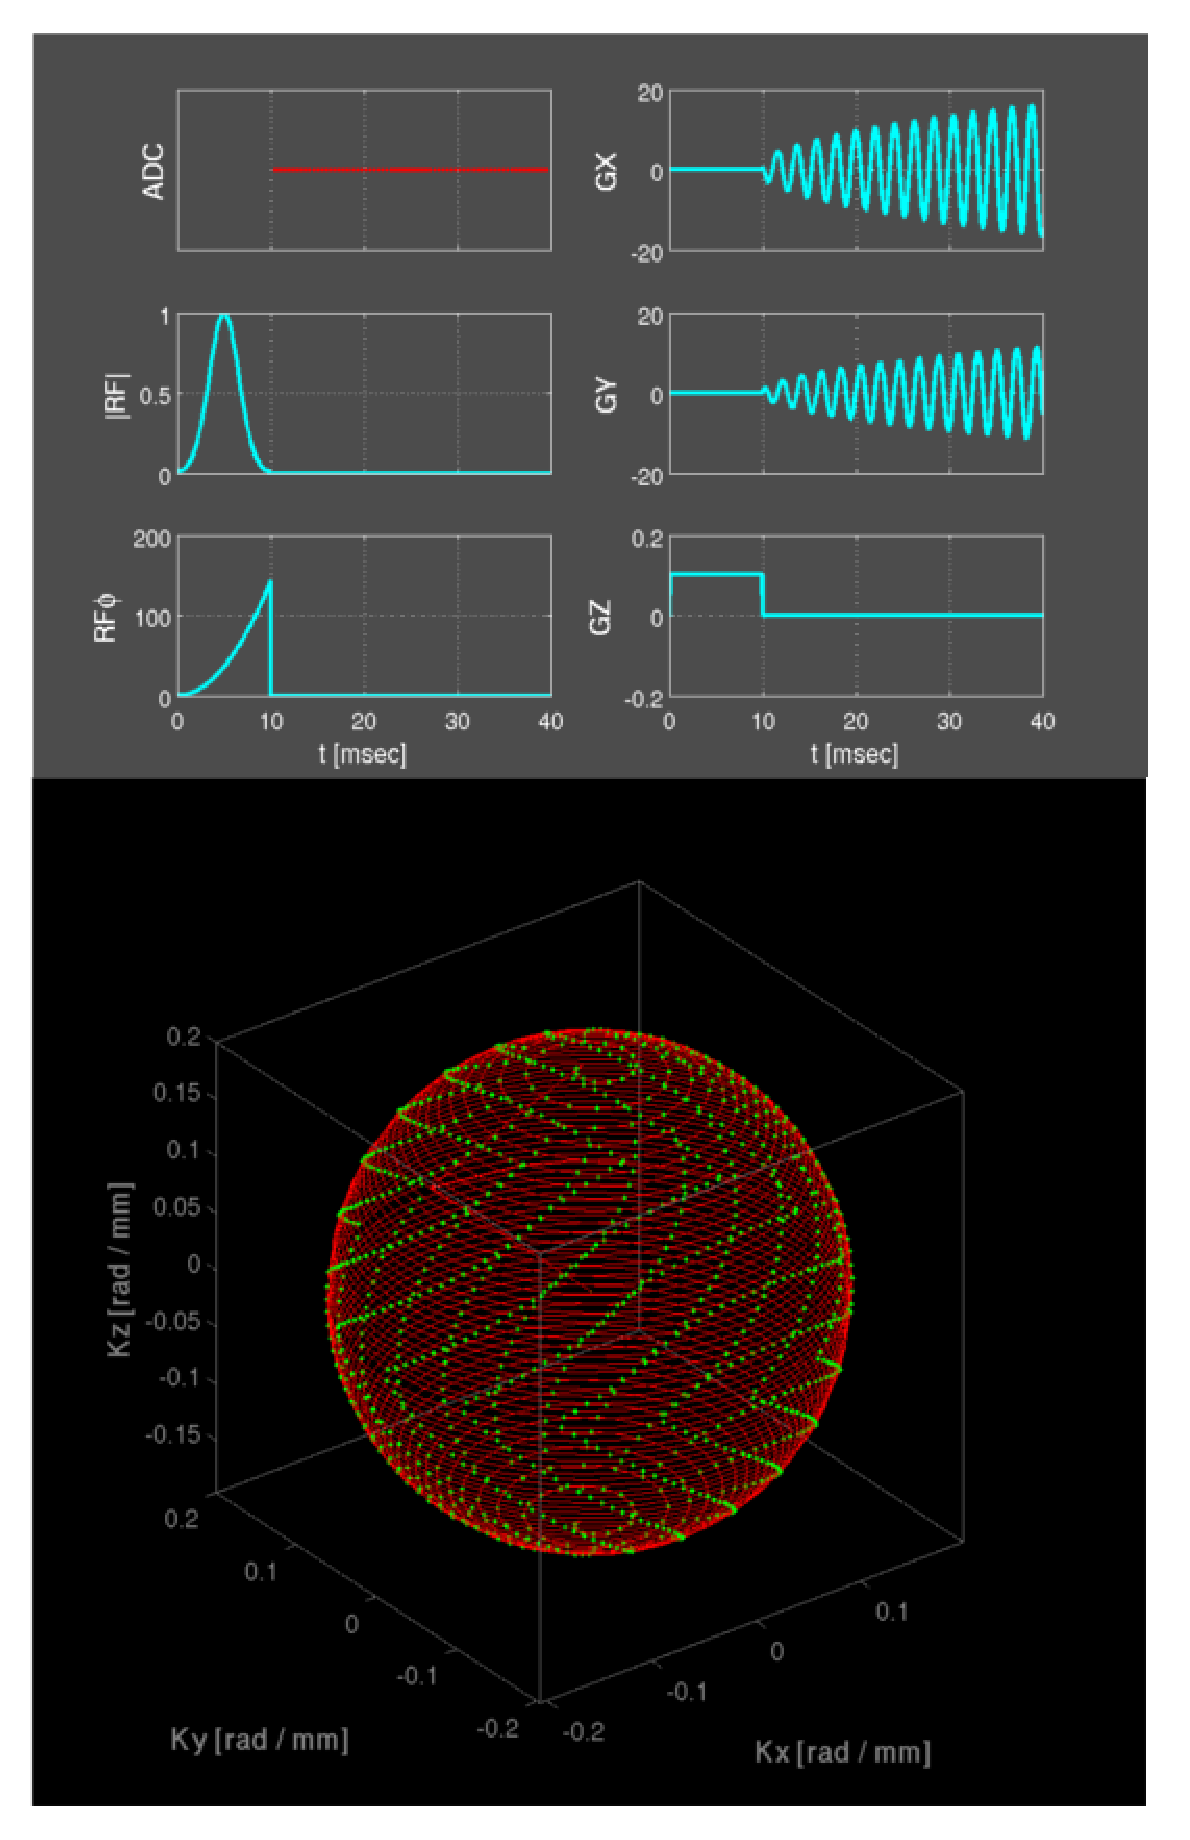
\includegraphics[width=0.60\columnwidth]{fig/SeqDiagTrajectExmpl.eps}}\\
  \subfigure[RF Coil Layout]{\label{fig:guisc}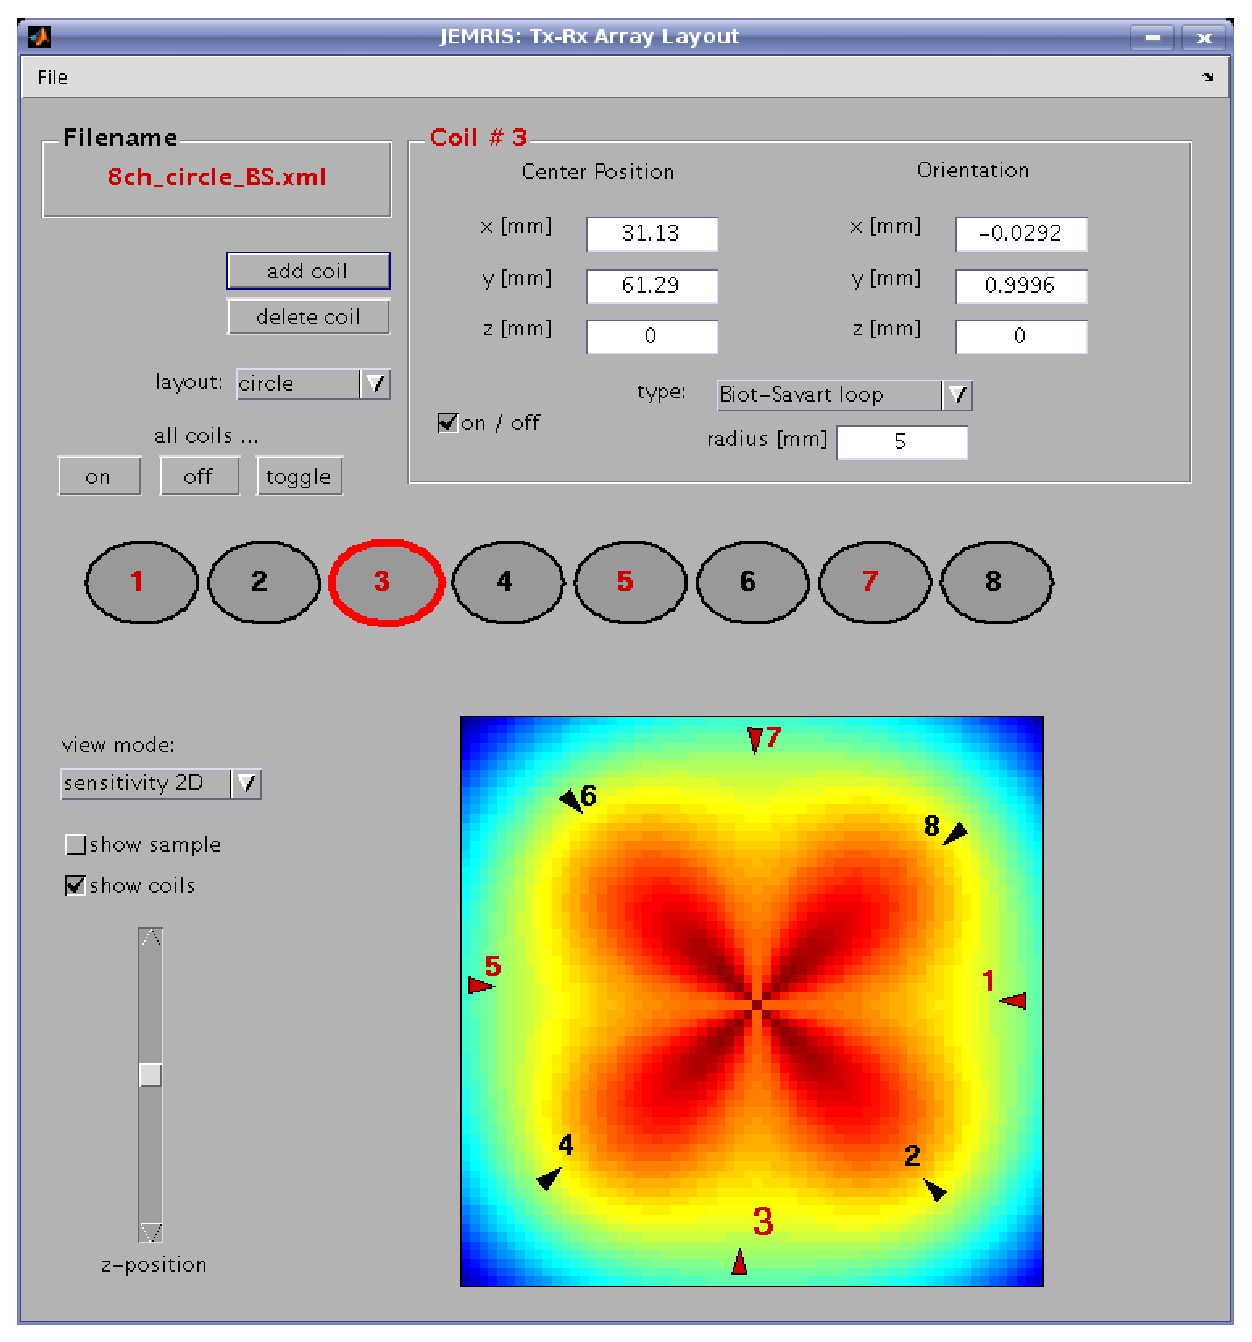
\includegraphics[width=0.88\columnwidth]{fig/guiTxRx.eps}}
  \hfil
  \subfigure[Simulation]{\label{fig:guisd}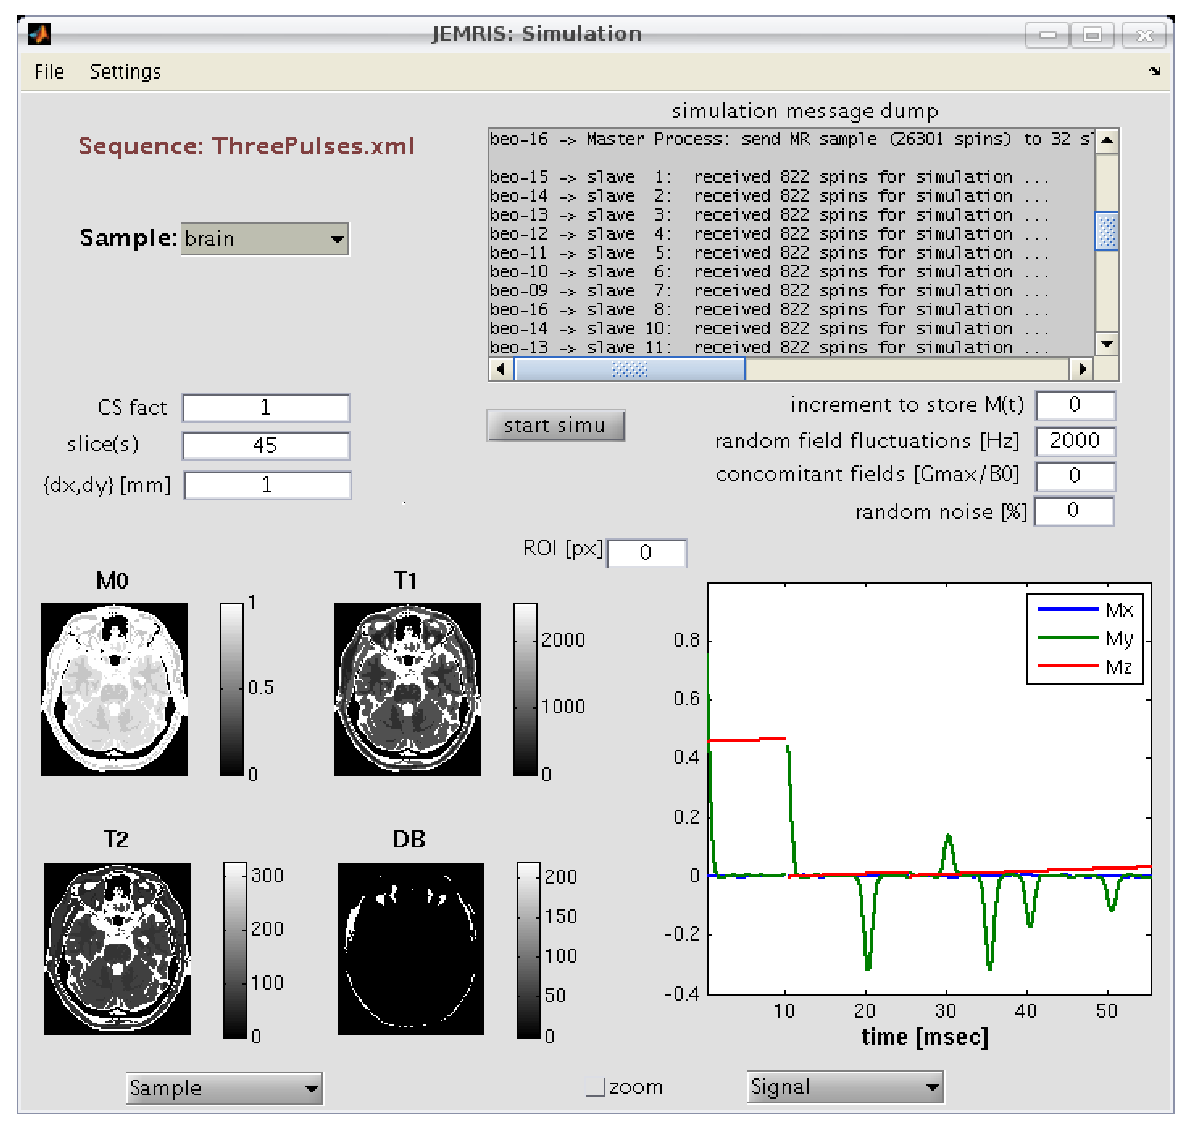
\includegraphics[width=1.0\columnwidth]{fig/guiSim.eps}}
 \label{fig:guis}
 \caption{JEMRIS GUI examples: \subref{fig:guisa} Sequence development of a CPMG imaging sequence. All modules are given
   in the top panel for tree insertion. Attributes of the selected node may be edited above the tree. Here, a
   phase-encode gradient which performs a linear phase encoding order according to the formula of the
   area-attribute. \subref{fig:guisb} {\it Top:} Example pulse sequence diagram produced by the GUI for the presentation
   of analytic pulses. None of these waveforms, the gradient spiral as well as the frequency sweep, are explicitly part
   of the framework.  \subref{fig:guisb} {\it Bottom:} K-space trajectory plotted by the sequence GUI for a spherical
   navigator. Green dots mark the points of data acquisition. \subref{fig:guisc} RF coil array layout example with eight
   elements of which 4 are marked as active. \subref{fig:guisd} Simulation of a simple three pulse sequence (
   60$^\circ$-90$^\circ$-90$^\circ$ at 0-10-25 ms) on the human brain phantom under strong field inhomogeneities results
   in the famous five echoes: three spin echos, one reflected spin echo, and the stimulated echo.}
\end{figure*}

%\twofig{fig/guiSimu.tif}{fig/guiTxRx.tif}{Example of the JEMRIS GUI for simulations:


%%%%%%%%%

\subsection{Examples}\label{ssec:ex}

\subsubsection{MRI Artefact Simulations}

Simulations were performed on 60,000 spins of the human head model; the calculation times with 32 compute nodes of the
cluster were 1 minute for the EPI experiments and 10 minutes for the TrueFISP and the spin echo experiment,
respectively.  The results of image artefact generation are given in Fig.~\ref{fig:artefacts}: a) EPI simulation
considering chemical shift effects yield the prominent fat-water shift in MRI; b) malfuncting MR scanner hardware
simulation with a nonlinear gradient field results in a distorted EPI image; c) TrueFISP simulation including
susceptibility-induced field inhomogeneity yields the well-known banding artefacts in the human brain; d) artefact in
spin echo imaging due to a very long inversion pulse exciting transverse magnetisation. Note that the latter example
cannot be realised with any simulator relying on analytical solutions of the Bloch equation due to neglect of relaxation
effects during the RF pulse. The exact simulation of the simultaneous occurrence of RF pulses and imaging gradients with
JEMRIS is the foundation for the investigation multidimensional selective excitation.\\ 

\epsfig{fig/artifacts.eps}{Example of artefact simulations on a human head model: {\bf a)} EPI with chemical shift; {\bf
    b)} EPI distortions due to a nonlinear read gradient; {\bf c)} TrueFISP banding artefacts (close to the eyes)
  resulting from susceptibility-induced field inhomogeneities; and {\bf d)} Artefact in a spin echo sequence with a long
  refocusing pulse in the order of $T_2$ of the sample.}{fig:artefacts}{tp}{1.0}


%%%%%%%%%%%%

\subsubsection{3D Selective Excitation}

Multidimensional, spatially-selective excitation \cite{pauly} is an important concept of growing interest in MRI,
e.g. in the field of {\it in vivo} spectroscopy or for the challenging task of correcting subject-induced $B_1$ field
inhomogeneities at ultra high fields \cite{ibrahim}. Currently, JEMRIS is being extensively used to design such pulse
and results will be published in the near future. Fig.~\ref{fig:selex} shows the capability of the software to correctly
simulate such experiments.  The corresponding RF pulse was calculated by means of the small tip-angle approximation for
the case of parallel transmission as described in \cite{ullmann}. The target pattern for selective excitation was,
following the good tradition with the literature, a checkerboard, however, a 3D variant. Eight transmit coils were
considered for this simulation.

\epsfig{fig/selex.eps}{Example of 3D simulated selective excitation. Note, that the simulator permits observation of the
  time course within the target pattern of selective excitation in addition to acquiring the image after
  excitation.}{fig:selex}{tp}{0.5}


%%%%%%%%%%%%%%%%%%%%%%%%%%%%%%%%%%%%%%%%%%%%%%%%%%%%%%%%%%%%%%%%%%%%%%%%%%%%%%%%%%%%%%%%%%%%%%%%%%%

\section{Conclusion}

This manuscript describes the new software environment JEMRIS which performs (classically) general MRI simulations
within reasonable calculation times. It is written in C++ and takes advantage of newly developed object-oriented design
patterns tailored for MRI sequence design and Bloch equation-based modelling of a large spin system under the influence
of different off-resonance effects. Thus, it allows time tracking of the net magnetisation, splitting of different
effects, and therefore accurate investigation of special MR samples (e.g.~implants) and new MRI sequences under a
variety of experimental conditions. The computationally demanding task is tailored for high performance computing
environments. However, since the problem is ideally suited for parallelisation and does not rely on high speed
connections between the compute nodes, it is possible to use JEMRIS e.g.~within a local area network of PCs. Such an
environment allows the computation of realistic 2D MRI simulation within a few minutes whereas 3D simulation are in the
order of hours or even days. Thus, super-computing centres are more appropriate for large 3D simulations with JEMRIS. On
the other hand, as prices reduce and availability increases continuously for HPC systems, might be only a matter of a
few years before super-computing is possible in nearly every research lab. JEMRIS was developed in a lean, modular and
extensible way and is provided as an open-source project with the perspective to gain from the input of the MRI research
community. Another aspect was usability: JEMRIS allows a GUI-based setup of complex MRI sequences in a few minutes
without any programming involved. It has already been tested with great success for undergraduate teaching where the
students where able to independently develop spin echo, gradient echo, and EPI sequences and to investigate properties
of the (simulated) imaging results all in a single practical day.  It is further intended to support the rapidly
evolving field of medical image processing which might benefit from a gold standard, serving as a test-bed for the
application of new methods and algorithms. Here, JEMRIS could provide a general framework for generating standardised
and realistic MR images for many different situations and purposes.\\

Future developments are already in progress in several research projects: for a complete control of the RF transmit and
receive processes, interfaces to already existing Maxwell-based simulators for RF coil design are under
evaluation. Additionally, there are strong efforts for generalised MRI simulation of dynamic processes in the sample,
such as brain perfusion and diffusion, especially to study more realistic simulations of functional MRI
experiments. From the implementation point of view, the software needs only little changes to account for time dependent
changes of isochromat positions. However, then the underlying physical models become much more demanding from the
computational point of view. Further, magnetisation transfer and the treatment of non-classically interacting spins are
currently under investigation. Another important effect in real experiments is the temporal non-ideal behaviour of the
gradient system, commonly termed as eddy currents, which are currently integrated in the present approach by an
analytical description of the gradient waveform \cite{barker}. Results of these and other projects will be integrated in
future releases of the freely available software. Finally, so far JEMRIS only acquires simulated MRI data but lacks the
image reconstruction part which is left to the user (although the simulation GUI has, for convenience, some basic FFT
functionality). A solid framework which integrates reconstruction to the present framework would be of interest.
This, however, it is not part of near future plans in J\"ulich -- it could be a task for contributing image processing
experts.

\section*{Availability}
JEMRIS is available from the official developer website \verb+http://www.jemris.org+.

\bibliographystyle{IEEEtran}
\bibliography{jemris_ref.bib} % commented if *.bbl file included, as
%\begin{thebibliography}{1}
%\end{thebibliography}


\end{document}


